\chapter{Introduction}\label{chap:Introduction}
Drones have a wide variety of potential uses, such as search and rescue, inspection, security, surveillance, research, aerial photography, unmanned cargo systems, military applications, etc. Drones are already widely used, and while some of the aforementioned applications raises ethical issues for debate, there is no doubt that drones also hold a place in the future.

Multicopters constitutes a class of drones with fixed-pitch propellers. This means that the actuation is achieved solely from a difference in speed between the propellers. Among all the different varieties of multicopters, see some examples in \autoref{fig:multicopters}, the quadcopter is the most popular, largely due to a compromise between stabilization capabilities and cost of hardware. \cite{TypesOfMulticopter}

\begin{figure}[H]
  \centering
  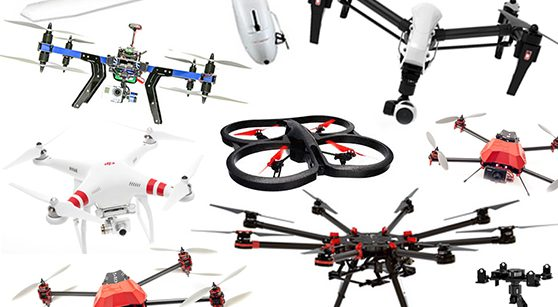
\includegraphics[width=.6\linewidth]{figures/multicopters}
  \caption{A small selection of drones which belongs to the large class of multicopters. \cite{multiCopterPhoto}}
  \label{fig:multicopters}
\end{figure}

The aim of the project is to investigate the capabilities of a specific design strategy when controlling a quadcopter as part of a distributed system.

The control of a quadcopter has been addressed many times in the recent years. One example is where the quadcopter is controlled using a back-stepping technique and non-linear controllers \cite{backstepping}. Another way of solving the control problem is where the quadcopter attitude is modeled using quaternions and controlled with a PD based non-linear controller \cite{quaternionsPD}. There is a multitude of possible solutions, and while non-linear control is a popular choice for quadcopters, this project addresses the possibility of using linear controllers and Euler angle representation.

The quadcopter obtains its attitude and position over a network from an external motion tracking system. This introduces delay and packet loss as a limiting factor to the control system situated on the quadcopter. The controlling code is implemented in C on a microcontroller using a real time operating system (RTOS), called FreeRTOS.

The system's coupled behavior and instability raises a challenging control task. This task is solved by implementing a controller design, which is based on a model derived by first principle modeling. This is later linearized since it is desired to use linear controllers.

The system is divided into an attitude controller and translational controllers. The attitude control strategy is based in state space design, and makes use of state feedback and integral control using LQR. The translational controllers are designed with classical control methods.

This project provides design and realization of the described system. Subjects in focus are the performance achievable using the chosen linear attitude control strategy, the influence of remote sensing, the influence of the attitude control bandwidth on the translational controllers and the performance of a cascaded control structure with classical linear translational controllers.

